\documentclass[11pt]{scrartcl}

\usepackage{ucs}
\usepackage[utf8x]{inputenc}
\usepackage[T1]{fontenc}
\usepackage[ngerman]{babel}
\usepackage{amsmath,amssymb,amstext}
\usepackage{graphicx}
\usepackage[justification=RaggedRight, singlelinecheck=false]{caption}
\usepackage{tikz}
\usepackage[square,sort,comma,numbers]{natbib}


\title{Fortgeschrittenen Praktikum Teil 1: IKF}
\subtitle{Versuch 1: $\gamma \gamma$ - Koinzidenzen \\ Betreuer: Alexander Schottelius}

\author{Gruppe 1: Reinhold Kaiser, Florian Stoll}

\date{14.04.2018}

\begin{document}
\maketitle
\newpage
\tableofcontents
\newpage
\bibliographystyle{alphadin}

\section{Zielsetzung}
In dem Versuch $\gamma$-$\gamma$-Koinzidenzen sollen für zwei Beispiele die Winkelverteilung zweier gleichzeitig entstehender Photonen
gemessen werden. Zum Einen entsteht beim Betazerfall von $^{22}Na$ ein Positron, welches wiederum mit
einem Elektron zu zwei $\gamma$-Quanten annihiliert. Zum Anderen zerfällt $^{60}Co$ zu $^{60}Ni$
und dieses dann über Kaskaden in den Grundzustand. Dabei werden zwei $\gamma$-Quanten emittiert,
deren Winkelkorrelation gemessen werden soll. Physikalisch relevant sind die Messungen von 
Winkelverteilungen, weil durch sie auf die Spin- und Drehimpulsquantenzahlen der angeregten Zustände 
geschlossen werden kann.


\section{Theoretische Grundlagen}

\subsection{Wechselwirkungen elektromagnetischer Strahlung mit Materie}

Um $\gamma$-Strahlung nachweisen zu können macht man sich die Beobachtung der drei Wechselwirkungsprozesse von $\gamma$-Strahlung mit Materie zu Nutze. Diese Wechselwirkungsprozesse liefern, je nach Energiebereich und Detektormaterial, einen unterschiedlichen Beitrag zum gesamten Spektrum. Der Photoeffekt dominiert bei Photonenenergien im keV-Bereich, wohingegen der Compton-Effekt überwiegend im Bereich von 100 keV bis wenige MeV relevant ist. Der Paarbildungsprozess dominiert dagegen bei Energien im MeV-Bereich.

\paragraph{Der Photo-Effekt}

Beim Photoeffekt wird ein Photon von einem Hüllenelektron absorbiert. Es kommt zum vollständigen Energieübertrag an das Elektron, wodurch es aus seiner Bindung mit dem Atomkern gelöst wird und das Atom verlässt. Damit dieser Vorgang stattfinden kann, muss die Energie $E_\gamma$ des einfallenden Photons größer sein als die Bindungsenergie $E_b$ des Elektrons. Je nachdem, in welcher Elektronenschale sich das Elektron befindet, variiert diese Bindungsenergie. Wegen der Impulserhaltung werden bevorzugt Elektronen aus den beiden innersten Schalen herausgelöst. Die kinetische Energie des emitierten Eletrkons folgt dabei der Beziehung

\begin{align}
E_{kin}=E_\gamma - E_b
\end{align}

Da nun in einer der energetisch niedrigeren Schalen ein Elektron fehlt, tritt an dessen Stelle ein Elektron aus einem energetisch höheren Niveau. Die dabei freiwerdende Energie wird in Form eines charakteristischen Photons abgestrahlt. Begünstigt wird der Photoeffekt durch eine Ordnungszahl des Targetatoms und niedrige Photonenenergien.

\paragraph{Der Compton-Effekt}

Trifft ein Photon auf ein schwach gebundenes Elektron eines Atoms, so wird durch einen elastischen Stoß ein Teil seines Impulses und seiner Energie auf dieses Elektron übertragen. Das Elektron verlässt das Atom, während das gestreute Photon an Energie verliert. Der Energieverlust des gestreuten Photons führt zu einer Frequenzänderung. Je nach Streuwinkel verändert sich dieser Energieübertrag an das Photon. Bei einer Streuung um $180^\circ$ wird der Übertrag maximal. Der Wirkungsquerschnitt steigt dabei mit zunehmender Kernladungszahl und nimmt mit steigender Photonenenergie ab. 

\subsection{Die Paarvernichtung}
Wie jedes Elementarteilchen besitzt auch das Elektron ein Anti-Teilchen mit gleichem Spin und gleicher Ruhemasse, jedoch mit entgegengesetzter Ladung. Dieses wird als Positron bezeichnet. Als Formelzeichen verwendet man hier $ e^{+} $ um die positive Ladung kennzuzeichnen. Dieses Positron kann als Nebenprodukt bei radioaktiven Atomkernen ( $\beta {^+} $ - Zerfall) oder durch die Paarbildung eines $\gamma $- Quants, das in ein Positron und eine Elektron zerfällt, entstehen. 
Die sogenannte Paarvernichtung ist der Umkehrprozess zur Paarbildung. Dabei wird ein Elektron-Positron-Paar wieder in elektromagnetische Strahlung umgewandelt. Dabei können jedoch unterschiedliche Anzahl an Photonen entstehen. Auch hier muss aber ein Stoß vorliegen, da sonst Impuls- und Energieerhaltung verletzt werden würden. Ein sogenannter Ein-Quanten-Zerfall, bei dem ein Paar tatsächlich nur in ein Photon umgewandelt wird, kann aus den gleichen Gründen nur bei einem Stoß mit einem Impuls- und Energieaufnahmefähigen Partner vorkommen, was nur im Festkörper vorkommt. Dieser Zerfall ist allerdings sehr unwahrscheinlich, und wird für diesen Versuch auch nicht berücksichtigt. 
Da das Elektron und das Positron beide den Spin $\frac{1}{2}$ haben, gibt es zwei verschiedene Einstellmöglichkeiten der Spins zueinander. Liegen die Spins parallel, besitzt das Paar einen Gesamtspin von 1, liegen sie anti-parallel ergibt sich ein Gesamtspin von 0. Der Grundzustand mit $S=0$ ist dabei nicht entartet, der Zustand mit $S=1$ ist dreifach entartet. Daraus ergibt sich eine Wahrscheinlichkeit von 3:1 für einen Zerfall des Triplett-Zustands, da die Wahrscheinlichkeiten für die Einstellmgölichkeiten der beiden Spins alle gleich sind. Die bei der Paarvernichtung entstehenden Quanten haben allerdings den Spin 1. Darum kann der Grundzustand nur in zwei $\gamma$ - Quanten zerfallen, während der Triplett-Zustand in drei Photonen zerfallen muss. Das stellt allerdings einen Prozess höherer Ordnung dar und ist daher deutlich unwahrscheinlicher. Im durchgeführten Versuch werden wir uns auch ausschließlich auf Paarvernichtungen aus dem Singulett - Zustand, d.h. mit zwei auftretenden $\gamma$ - Quanten beschränken.


\subsection{Betazerfall von $^{22}Na$ und $^{60}Co$}

Im ersten Versuchsteil soll die Winkelverteilung zweier bei der Paarvernichtung entstehenden Photonen gemessenen werden. Um die Paarvernichtung überhaupt darstellen zu können, wird neben den in der Materie vorhandenen Elektronen zumindest ein Positron benötigt. Hierfür wird der $\beta^+$-Zerfall von $^{22}Na$ genutzt. Prinzipiell zerfällt beim $\beta^+$-Zerfall ein Proton des Atomkerns in ein Neutron, ein Positron und ein Elektron-Neutrino:

\begin{align}
p \rightarrow n + e^+ + \nu_e
\end{align}

Dabei emittiert in unserem Fall das $^{22}$Na  ein Positron und ein (nicht messbares) Neutrino und geht in einen angeregten Neon-Kern über. Dieser strahlt nach kurzer Zeit ein weiteres $\gamma$-Quant mit einer Energie von 1275keV ab und geht in den Grundzustand als $^{22}$Ne über. In Abbildung \ref{Na22} ist das Zerfallsschema nochmal dargestellt.

Im zweiten Versuchsteil untersuchen wir eine $^{60}$Co-Probe, welche durch $\beta^-$-Zerfall in einen angeregten $^{60}$Ni-Kern zerfällt. Bei der Abregung sind zwei $\gamma$-Übergänge möglich, durch die zwei Photonen mit den Energien von 1,172 MeV und 1,33 MeV ausgesandt werden. Da der Zwischenzustand mit einer Lebensdauer  von $10^{-12}$s sehr kurzlebig ist, treten die beiden Quanten quasi gleichzeitig auf. In Abbildung \ref{Co60-bild} ist das zugehörige Termschema ebenfalls dargestellt.



\begin{figure}[htbp] 
	\begin{minipage}[t]{0.45\linewidth} 
     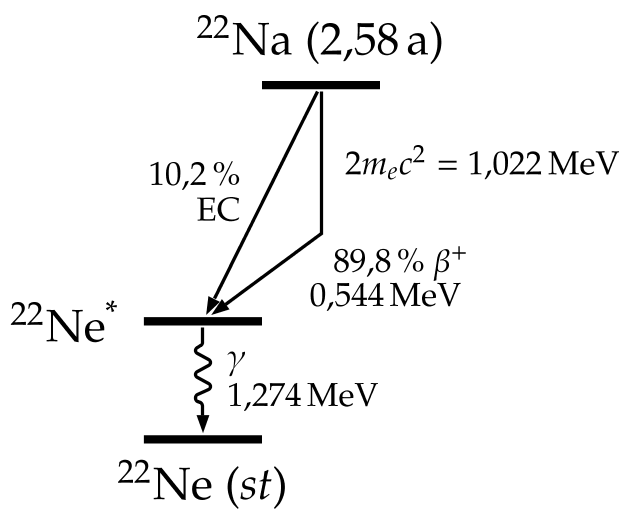
\includegraphics[width=1\textwidth]{Na22.png}
  \caption{Zerfallsschema von $^{22}$Na}
  \label{Na22}
\end{minipage}
\hfill
\begin{minipage}[t]{0.45\linewidth}  
     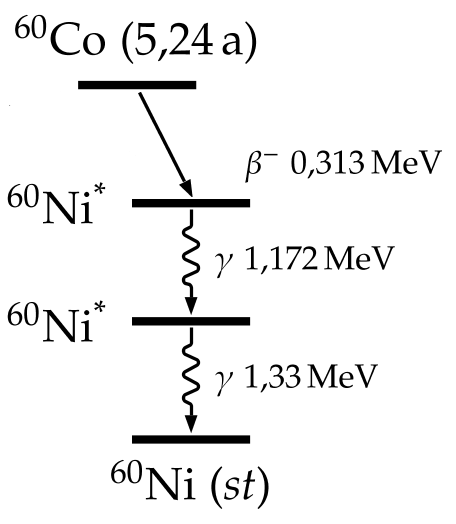
\includegraphics[width=0.7\textwidth]{Co60.png}
  \caption{Zerfallschema von $^{60}$Co}
  \label{Co60-bild}
\end{minipage}


\end{figure}

\subsection{Koinzidenztheorie}
Eine Koinzidenz ist dann vorhanden, wenn zwei Detektoren
innerhalb eines Zeitintervalls, der Koinzidenzzeit, beide ein 
Signal messen. Unterschieden werden muss dabei zwischen den 
wahren Koinzidenzen und den zufälligen Koinzidenzen. Bei den wahren
Koinzidenzen können die beiden Signale einem einzigen physikalischen
Prozess zugeordnet werden. Die zufälligen Koinzidenzen entstehen
durch Detektion zweier Teilchen, die durch unabhängige physikalische
Vorgänge innerhalb der Koinzidenzzeit emittiert wurden. Im Experiment
soll erreicht werden, dass das Verhältnis von wahren zu zufälligen 
Koinzidenzen möglichst hoch ist, was durch geeignetes Wählen der 
Versuchsbedingungen erreicht wird.

Des Weiteren wird eine möglichst hohe Koinzidenzrate angestrebt. 
Die Einzelzählraten der beiden Detektoren ergeben sich aus
\begin{equation}
 Z_i=\varepsilon_i \omega_i Q, \;\;\; i=1,2,
\end{equation}
wobei $\varepsilon_i$ die Ansprechempfindlichkeit ist, $\omega_i$
der Raumwinkel, unter dem der Detektor die Signalqualle sieht und
$Q$ die Zerfallsrate der Probe \cite{versuch}. 

Um die Koinzidenzrate zu erhalten, muss die Zählrate des 1. Detektors
mit der Wahrscheinlichkeit multipliziert werden, dass der 2. 
Detektor ein Signal registriert. Diese Wahrscheinlichkeit kann 
vom Winkel abhängen, unter dem beide Signale gemessen werden, daher
wergibt sich für die Wahrscheinlichkeit einer Koinzidenz mit der 
Winkelverteilung $W(\vartheta)$:
\begin{equation}
 P(\vartheta)=\epsilon_2\omega_2 W(\vartheta)
\end{equation}
Die echte Koinzidenzrate ist daher:
\begin{equation}
 Z_{eK}=\varepsilon_1 \omega_1 \varepsilon_2 \omega_2 Q W(\vartheta)
\end{equation}

Um die Rate der zufälligen Koinzidenzen zu erhalten, betrachtet man die Wahrscheinlichkeit, dass
nach dem Messen von Detektor 1 innerhalb der Koinzidenzzeit $\tau$ ein unkorreliertes Signal im Detektor 2 
gemessen wird: $Z_2\cdot \tau$

Die Rate zufälliger Koinzidenzen ist daher:
\begin{equation}
 Z_{zK}=\tau Z_1Z_2
\end{equation}
Und das Verhältnis von echten zu zufälligen Koinzidenzen ist dann:
\begin{equation}
 \frac{Z_{eK}}{Z_{zK}}=\frac{1}{\tau Q}
\end{equation}
Für die Versuchsbedingungen bedeutet das, die Koinzidenzzeit so gering wie möglich zu wählen.
Außerdem sollten eine radioaktive Probe genutzt werden, deren Zerfallsrate nicht zu hoch ist,
aber dennoch nicht so gering,
dass man mit einem akzeptablen Zeitaufwand ein statistisch relevantes Ergebnis erhält.

\subsection{$\gamma$-$\gamma$-Winkelkorrelation}
Entstehen bei einem radioaktiven Zerfall oder einer Annihilation zwei Gamma-Quanten, sind sie
in ihrem Winkel zueinander korreliert. Das heißt, dass es eine Winkelverteilung der Intensität
der Koinzidenzen gibt, die charakteristisch für diese Art Zerfall ist. 

Der einfachste Fall ist die Annihilation von Positron und Elektron, bei der Gesamtimpuls von $~0$ 
erhalten bleibt. So werden die Gamma-Quanten unter einem Winkel von $180^\circ$ zueinander gemessen.

Im Fall eines Kerns, der über eine Kaskade von 2 Gamma-Quanten zerfällt wird die Annahme gemacht, dass
die Lebensdauer des Zwischenzustands so kurz ist, dass sich die Orientierung des Kerns im Vergleich 
zum ersten Zerfall nicht verändert. 

Allgemein kann die Winkelverteilung über die Formel
\begin{equation}
 W(\theta)=\sum_\nu A_\nu^{(1)} A_\nu^{(2)} P_\nu ( \cos \theta)
\end{equation}
angegeben werden \cite{grundlagen}. Dabei sind die $A_\nu^{(i)}$ Koeffizienten, die aus Tabellen abgelesen werden können.
$P_\nu(\cos \theta)$ sind Legendre-Polynome der $\nu$-ten Ordnung, wobei für nicht-polarisierte Strahlung
allerdings nur geradzahlige Polynome in der Winkelverteilung auftreten. Dadurch treten nur geradzahlige
Potenzen von $\cos \theta$ auf, was die Winkelverteilung $W(\theta)$ zu einer zu $90^\circ$ symmetrischen
Funktion macht. Es reicht daher die Messung auf einen Bereich von $\theta=0^\circ$ bis $90^\circ$ zu 
beschränken.

Die ersten drei relevanten Legendre-Polynome nehmen folgende Form an:
\begin{eqnarray}
 P_0 &=&1\\
 P_2 & = & \frac{1}{2}(3 \cos^2 \theta - 1)\\
 P_4 &=& \frac{1}{8}(35\cos^4 \theta - 30 \cos^2 \theta +3)
\end{eqnarray}

Durch Einsetzen der passenden Koeffizienten $A_\nu^{i}$ erhält man dann Winkelverteilungen für
einige $\gamma$-$\gamma$-Kaskaden, die in Abbildung \ref{winkelvert} dargestellt sind.

\begin{figure}[htbp]  
     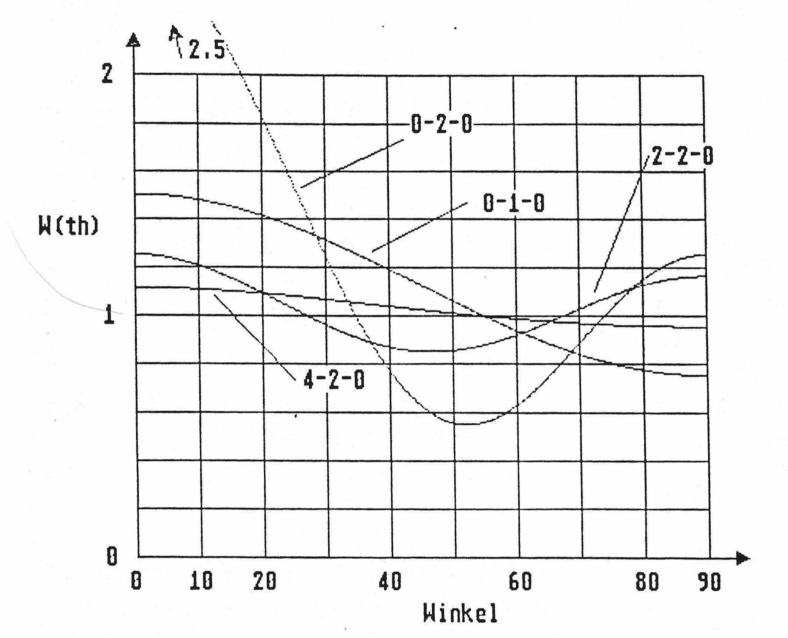
\includegraphics[width=0.7\textwidth]{Winkelverteilung.pdf}
  \caption{Winkelkorrelationen für einige $\gamma$-$\gamma$-Kaskaden \cite{versuch}}
  \label{winkelvert}
\end{figure}

Von speziellem Interesse für den Zerfall von $^60$Co ist die Winkelkorrelationsfunktion der 
$4-2-0$-Kaskade. Sie wird hier einmal als Formel ausgeführt, um die theoretische Winkelkorrelation
mit der gemessenen zu vergleichen \cite{versuch}.

\begin{eqnarray}
 W(\theta)&=&P_0+0.1020\cdot P_2+0.009087 P_4\\
 &=&1+0.1020\cdot \frac{1}{2}(3 \cos^2 \theta - 1)+0.009087\cdot \frac{1}{8}(35\cos^4 \theta - 30 \cos^2 \theta +3)
 \label{winkelverteilung}
\end{eqnarray}


\subsection{Fehlerrechnung}

Wie jede Messung ist auch der durchgeführte Versuch nicht frei von fehlerbehafteten Größen. Da wir keine genaueren Angaben treffen können, gehen wir von normalverteilten Größen aus, deren Fehler sich in erster Näherung wie folgt berechnen lässt:

\begin{align}
\Delta N = \sqrt{N}
\end{align}

Mithilfe dieser Formel werden alle im Folgenden angegebenen Fehler abgeschätzt. Damit decken wir einen Bereich von $1\sigma$ ab, das heißt der wahre Wert liegt mit einer Wahrscheinlichkeit von $66,67\%$ innerhalb unseres Fehlerbereichs. 

\section{Versuchsaufbau und Messgeräte}

Zum Nachweise der $\gamma$-Strahlung werden in diesem Versuch zwei NaI-Szintillationszähler verwenden. Dieser besteht prinzipiell aus einem Szintillator und einem Photomultiplier und ist schematisch in Abbildung \ref{PMT} dargestellt. Treffen energiereiche Photonen auf den Szintillationskristall, so werden durch die oben beschriebenen Wechselwirkungsprozesse Elektronen ausgelöst. Diese können Atome im Kristall anregen oder ionisieren, wodurch Fluoreszenzphotonen emittiert werden. Die vom Szintillator emittierten Photonen werden über einen Lichtwellenleiter an einen Photomultipliert weitergeleitet und schlagen in diesem über den Photoeffekt Elektronen aus den Atomen, welche kaskadenartig über eine zwischen einer Vielzahl an Dynoden angelegten Spannung vervielfacht und in ein messbares Signal umgewandelt werden. Als Szintillationskristall dient in unserem Fall ein mit Thallium dotierter Natriumiodid-Kristall. Die Thalliumatome dienen als Leuchtzentren im Szintillator. Ihre Anregungsenergie liegt innerhalb der Bandlücke des Natriumiodids, wodurch sie leichter angeregt werden können, was wiederum in einer guten Photonenausbeute im sichtbaren Bereich resultiert. Die Größe des Kristalls wird bei Szintillatoren so gewählt, dass die Wahrscheinlichkeit für die genannten Wechselwirkungsprozesse ausreichend groß ist. 

\begin{figure}[htbp]  
     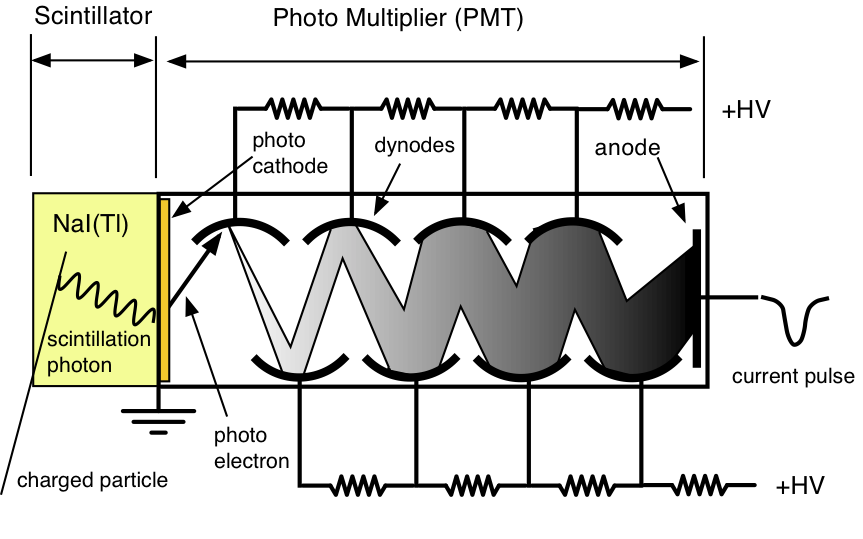
\includegraphics[width=0.7\textwidth]{PMT.png}
  \caption{Schematischer Aufbau eines NaI-Szintillationszählers}
  \label{PMT}
\end{figure}

\begin{figure}[htbp]  
     \usetikzlibrary{shapes,arrows}
\tikzstyle{block1} = [draw, fill=blue!20, rectangle, 
    minimum height=3em, minimum width=4em, text width=1cm]
\tikzstyle{block2}=[draw, fill=blue!0,rectangle, minimum height=3em, minimum width=4em, text width=1cm]
\tikzstyle{lense} = [draw, fill=blue!00, ellipse, 
    minimum height=6em, minimum width=2em]
\tikzstyle{filter}=[draw, fill=black!40,rectangle, minimum height=4.5em, minimum width=0.3em]
\begin{tikzpicture}
\coordinate (O) at (0,0);
\coordinate (L0) at (-7,0);
\coordinate (L1) at (-4,0);
\coordinate (R0) at (2,0);
\coordinate (R1) at (2.5,0);
\coordinate (R2) at (3,0);
\coordinate (R3) at (4,0);
\coordinate (R4) at (7,0);

\node[block1, name=det] at (L0) {Photo-Det.};
\node[lense, name=lense1] at (L1){};
\node[block2, name=cell] at (O){Rb-cell};
\node[filter, name=f1] at (R0){};
\node[filter, name=f2] at (R1){};
\node[filter, name=f3] at (R2){};
\node[lense, name=lense2] at (R3){};
\node[block1, name=lamp] at (R4){Lamp};
\draw (L0) -- (R4);
\draw (L0) -- (-4,1) -- (4,-1) -- (R4);
\draw (L0) -- (-4,-1) -- (4,1) -- (R4);
\end{tikzpicture}
  \caption{Schematischer Aufbau der Koinzidenmessung}
  \label{PMT2}
\end{figure}

\begin{figure}[htbp]  
     \usetikzlibrary{shapes,arrows}
\tikzstyle{block} = [draw, fill=blue!20, rectangle, 
    minimum height=2em, minimum width=4em]
\tikzstyle{sum} = [draw, fill=blue!20, circle, node distance=1cm]
\tikzstyle{input} = [coordinate]
\tikzstyle{output} = [coordinate]
\tikzstyle{pinstyle} = [pin edge={to-,thin,black}]
\begin{tikzpicture}[auto, node distance=2cm]

\node  [block, name=det1, label={[]above:fix}] {Det1};
\node [block, right of= det1] (pm1) {PM};
\node [block, below of=det1, name=det2,  label={[]below:bewegl.}] {Det2};
\node [block, right of= det2] (pm2) {PM};
\node [block, above of=pm1, name=volt1] {1000V};
\node [block, below of=pm2, name=volt2] {700V};

\draw [-] (det1) -- node[] {} (pm1);
\draw [-] (det2) -- node[] {} (pm2);
\draw [-] (volt1) -- node[] {} (pm1);
\draw [-] (volt2) -- node[] {} (pm2);

\node [block, name=ddl1, right of=pm1, node distance=3cm] {DDL AMP};
\node [block, name=ddl2, right of=pm2, node distance=3cm] {DDL AMP};
\node [block, name=tsca1, right of=ddl1, node distance=3cm] {TSCA};
\node [block, name=tsca2, right of=ddl2, node distance=3cm] {TSCA};

\draw [-] (pm1) -- node[] {} (ddl1);
\draw [-] (ddl1) -- node[name=line1] {} (tsca1);
\draw [-] (pm2) -- node[] {} (ddl2);
\draw [-] (ddl2) -- node[] {} (tsca2);


\node[block, name=adc, right of=tsca2, node distance=4cm] {ADC};

\node [block, name=time, above of=tsca1, node distance=3cm, align=center, xshift=1.5cm]{Time\\ Analyzer};
\node [input, name=node1, above of=line1, node distance=1cm] {};
\draw[-] (tsca1) |- node[label={[rotate=90, text depth=-1ex, xshift=-2cm]right:Start}] {}  (time);
\node [block, name=delay, above of= adc, node distance=3cm]{Delay};
\draw[-] (time) |- node[label={[rotate=0, text depth=2ex]right:Stop}]{} (delay);

\node [input, name=node2, below of=time, node distance =4cm]{};
\draw[-] (delay) |- node[]{} (node2) -| node[]{} (tsca2);

%\draw[-] (tsca1) -| node[]{} (adc);
\draw[-] (tsca2) -- node[]{} (adc);
\node [block, name=pc, right of=adc]{PC};
\draw[-] (adc) -- node[]{} (pc);

\node[block, name=count, above of =pc]{Counter};
\draw[-] (time) -| node[]{} (count);
\draw[-] (tsca1) -- node[]{} (count);

\node [input, name=node3, below of=tsca2, node distance =1.5cm]{};
\draw[-] (ddl2) |- node[]{} (node3) -| node[]{} (adc);



\end{tikzpicture}
  \caption{Blockschaltbild der Analyse-Elektronik}
  \label{PMT3}
\end{figure}

Die beiden Detektoren sind gemäß Abbildung \ref{PMT3} mit einer komplexen Analyse-Elektronik verschaltet. Das Signal der Detektoren wird dabei zunächst in einem sogenannten DDL-Amplifier vorverstärkt, bevor es in den sogenannten Timing Single Channel Analyzer (TSCAs) je nach Signalstärke in einzelnen Kanälen als Ereignis gezählt wird. An den TSCAs sind Einstellungen zu einer sogenannten Energieschwelle bzw. einem Energiefenster wählbar, über welche nur Ereignisse mit einer bestimmten Mindestenergie bzw. in einem bestimmten Energiebereich als Ereignis gezählt werden. Dafür können entweder der Counter oder über ein Analog-Digital-Wandler (ADC) der PC verwendet werden, über den man sich die kompletten Spektren der Detektoren anzeigen lassen kann. Um nun aus den Einzelzählungen der Detektoren eine Koinzidenzmessung zu realisieren, werden die beiden Ausgangssignale der TSCAs als Start und Stop-Signal eines Time Analyzers verwendet, welcher die Dauer zwischen Start- und Stop-Signal in seine Ausgangsimpulshöhe umwandelt. Ereignisse mit einer definierten maximalen Zeitdifferenz werden anschließend in einem Counter gezählt und stellen später unsere Koinzidenzereignisse dar. Über eine zusätzliche Delay-Box können die Signale gezielt verzögert werden, was für die Zeitauflösung und die Einstellung der Koinzidenzzeit wichtig wird. 

\section{Versuchsteil 1: Koinzidenzmessung von 511keV-Vernichtungsquanten bei Paarvernichtung}
Im ersten Versuchsteil soll die Winkelverteilung der bei der Paarvernichtung entstehenden Photonen gemessen werden. Diese sollten aufgrund der Impulserhaltung in einem Winkel von 180$^\circ$ auseinander fliegen, d.h. die Winkelverteilung müsste bei 180$^\circ$ ein scharfes Maximum an Koinzidenz-Ereignissen aufweisen. Zuvor müssen jedoch die Spektren der einzelnen Detektoren analysiert und eine Koinzidenzzeit festgelegt werden, innerhalb derer die Detektoren ein $\gamma$-Quant messen müssen, um ein wahres Koinzidenzereignis zu zählen. 

\subsection{Durchführung}
Zu Beginn des Versuchs werden jeweils die Einzelspektren der beiden Detektoren aufgenommen und über die Messelektronik im PC ausgegeben. Die Spektren weisen jeweils zwei Peaks auf, welche den entstehenden Gammaquanten einerseits der Paarvernichtung bei 511keV und andererseits der Abregung des Ne-Kerns bei 1275keV entsprechen. Über die Elektronik werden die Zählraten jedoch nicht in Energien, sondern in Kanälen angegeben. Diese müssen nach Aufnahme der Spektren noch in Energien umgerechnet werden, um die Energie-Eichung des Aufbaus bestimmen zu können. Die beiden aufgenommenen Spektren finden sich in den Abbildungen \ref{Na-beweg} und \ref{Na-fixed}. Für die beiden Detektoren liegen unterschiedliche Spannungsversorgungen vor, wobei auch die Verstärkungseinstellungen in den zugehörigen DDL-Vorverstärkern unterschiedlich gewählt werden musste, um ein vergleichbares Spektrum zu erhalten und alle Ereignisse zu messen. Aus den gemessenen Werten für die Lage der Peaks kann nun die Eichung der Zähler gemäß folgender Gleichung bestimmt werden:

\begin{align}
E_\gamma = a + b \cdot K
\end{align}

Die gewählten Parameter, wie auch die Kanallage der Peaks und die sich daraus ergebende Energieeichung finden sich in Tabelle \ref{para}. 

\begin{table}[h]
	\caption{Messparameter der Detektoren}
	\begin{tabular}{|c|c|c|c|c|c|c|c|}
	\hline
	 & Spannung & Course Gain & Fine Gain & Peak 1 & Peak 2 & a & b\\ \hline
	 Fixed Detektor & 700V & 4 & 4.2 & 339 & 1432 & 274,04 keV & 0,70 $\frac{keV}{K}$\\ \hline
	 Bewegl. Detektor & 1030V & 6.4 & 9.1 & 596 & 1499 & 6,74 keV & 0,85 $\frac{keV}{K}$\\ \hline
	\end{tabular}
\label{para}
\end{table}

\begin{figure}[htbp]  
     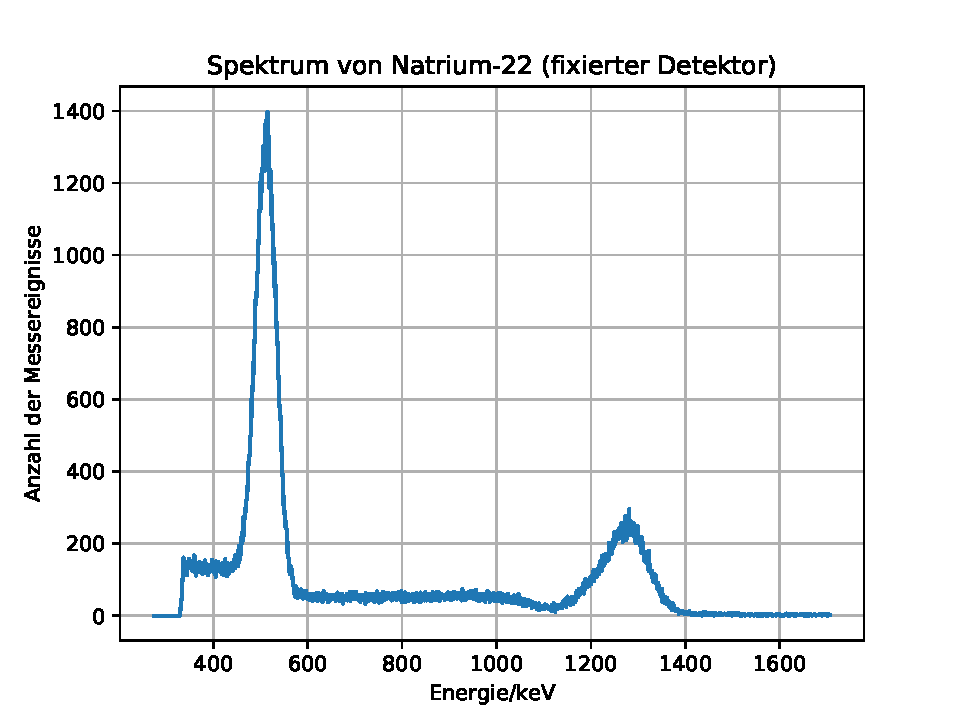
\includegraphics[width=0.7\textwidth]{Spektrum_von_Natrium-22_(fixierter_Detektor).pdf}
  \caption{Spektrum Na-22 des fixierten Detektors}
  \label{Na-fixed}
\end{figure}

\begin{figure}[htbp]  
     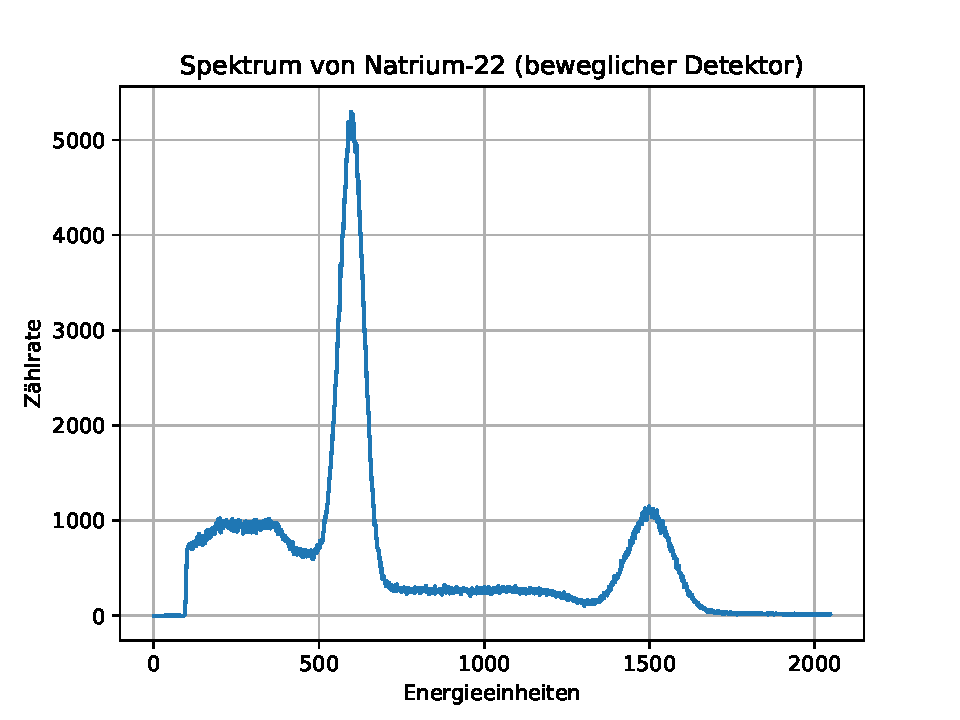
\includegraphics[width=0.7\textwidth]{Spektrum_von_Natrium-22_(beweglicher_Detektor).pdf}
  \caption{Spektrum Na-22 des beweglichen Detektors}
  \label{Na-beweg}
\end{figure}

Nun muss noch die Koinzidenzzeit der beiden Detektoren festgelegt werden. Dafür muss zunächst die Zeitauflösung der Anordnung bestimmt werden, um keine Ereignisse zu verpassen. Dafür werden an den beiden TSCAs die Energiefenster so eingestellt, dass ausschließlich die den 511-$\gamma$-Quanten zugehörigen Peaks zu sehen sind und die so entstandenen Ausgangssignale dem Time-Analyzer zugeführt. Dieser wandelt die Zeitdifferenz zwischen den beiden Signalen in die Impulshöhe seines Ausgangssignals. Um die Zeitauflösung zu bestimmen, wird das Ausgabesignal des Time-Analyzers als Spektrum angezeigt. Dabei werden zwei Messungen durchgeführt, wobei bei der zweiten Messung eine Verzögerung von 96ns auf das Signal gelegt wird. Durch die Bestimmung der Kanallage der Peaks und die Bestimmung ihrer Halbwertsbreite kann so die Zeitauflösung der Koinzidenzmessung analysiert werden. Die aus den Abbildungen \ref{mitDelay} und \ref{ohneDelay} bestimmten Peaklagen und die zugehörige Verzögerungen finden sich in Tabelle \ref{zeit}. 

\begin{table}[h]
	\caption{Messparameter der Detektoren}
	\begin{tabular}{|c|c|c|}
	\hline
	 & Messung 1 & Messung 2\\ \hline
	 Mittlere Kanallage & 458 & 1204\\ \hline
	 Zeitl. Verzögerung & 0 ns & 96 ns\\ \hline
	\end{tabular}
\label{zeit}
\end{table}

\begin{figure}[htbp] 
	\begin{minipage}[t]{0.45\linewidth} 
     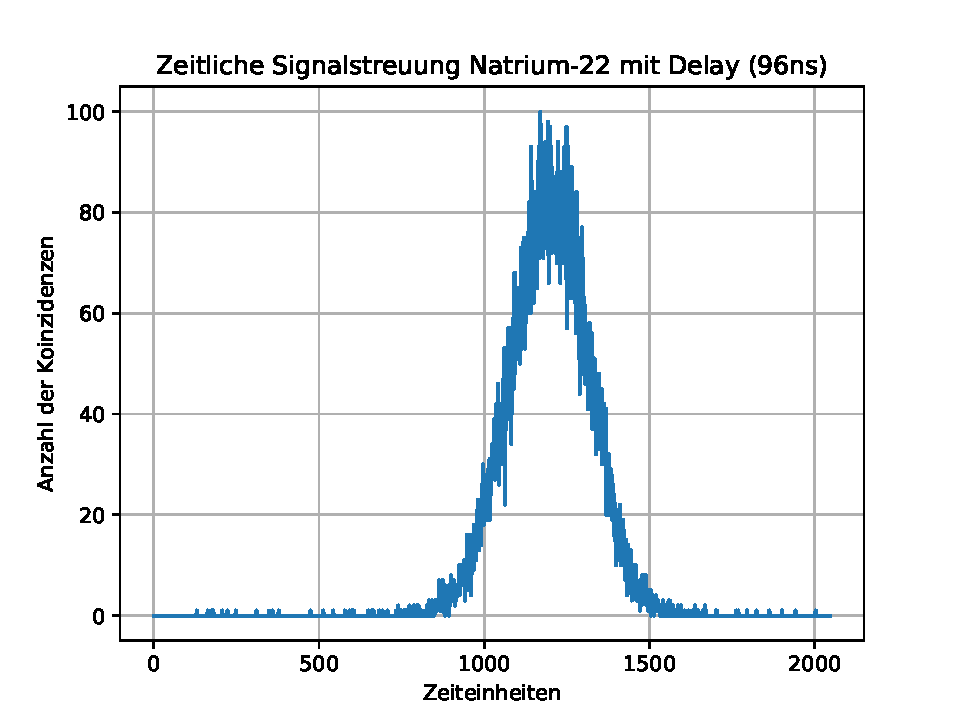
\includegraphics[width=1.2\textwidth]{Zeitliche_Signalstreuung_Natrium-22_mit_Delay_(96ns).pdf}
  \caption{Zeitliche Signalstreuung mit Delay}
  \label{mitDelay}
\end{minipage}
\hfill
\begin{minipage}[t]{0.45\linewidth}  
     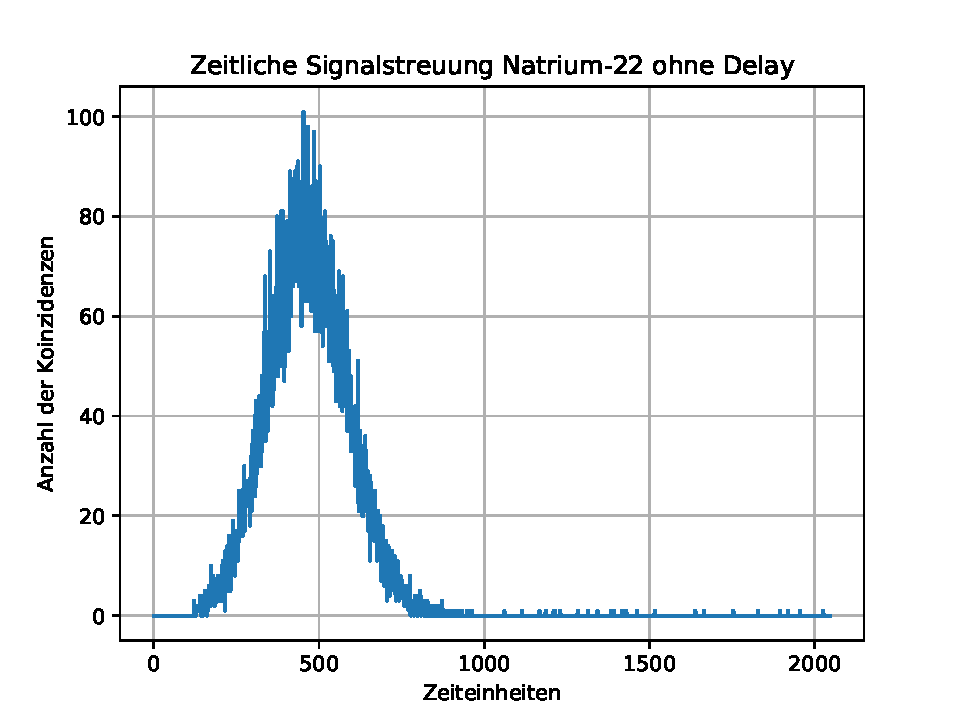
\includegraphics[width=1.2\textwidth]{Zeitliche_Signalstreuung_Natrium-22_ohne_Delay.pdf}
  \caption{Zeitliche Signalstreuung ohne Delay}
  \label{ohneDelay}
\end{minipage}
\end{figure}

Um die Winkelverteilung zu vermessen wird die Position des beweglichen Detektors in kleinen Schritten verändert und die entsprechende Koinzidenzrate aufgenommen. Aus den beiden Peak-Positionen und der gemessenen Halbwertsbreite von 273 Kanälen kann mit folgender Gleichung die Zeitauflösung bestimmt werden:
\begin{align}
\Delta t = \Delta K\cdot\frac{Delaytime}{K_{Delaytime=96ns} - K_{Delaytime=0}} = 273\cdot\frac{96ns}{1204-458}=35ns
\end{align}

Nun stellt sich ein weiteres Problem, da sichergestellt werden muss, dass das als Stop-Signal in den Time-Analyzer einfließende Signal des Detektors 1 nach dem als Start einfließenden Signal des Detektors 2 im Time-Analyzer ankommt. Um dies sicherzustellen und auch möglichst alle Koinzidenzereignisse im Time-Analyzer zu registrieren, wird mithilfe der Delay-Box eine zusätzliche Verzögerung auf das Stop-Signal geschaltet. Um wirklich alle Koinzidenz-Ereignisse zu messen und für jede das Stop-Signal definiert nach 
dem Start-Signal zu erhalten, wird diese auf 240ns eingestellt.

Da sich der Winkel des beweglichen Detektors am Messaufbau nicht direkt ablesen lässt, wird näherungsweise eine gerade Skala für die Position des Detektors verwendet und über den geometrischen Aufbau in Winkel umgerechnet. Dafür wird folgende Formel für die Beziehung des Abstands d zur Nullposition (Detektoren genau gegenüberliegend, Winkel 180$^\circ$) und den Drehwinkel $\alpha$ verwendet, wobei der Abstand der Quelle zum Detektor 635mm beträgt. 

\begin{align}
\alpha=\frac{\arcsin{\frac{d}{635mm}}}{2\pi}\cdot 360^\circ
\end{align}

Um weiterhin nur $\gamma$-Quanten zu messen, welche exakt in entgegengesetzter Richtung fliegen, wird um die Quelle in Richtung beider Detektoren eine Blei-Abschirmung angebracht, die nur einen sehr schmalen Spalt aufweist. Damit gelangen nur entgegengesetzt entstehende Photonen in die Detektoren und wir können unsere Koinzidenzmessung starten. 

\subsection{Auswertung}

\begin{figure}[htbp]  
     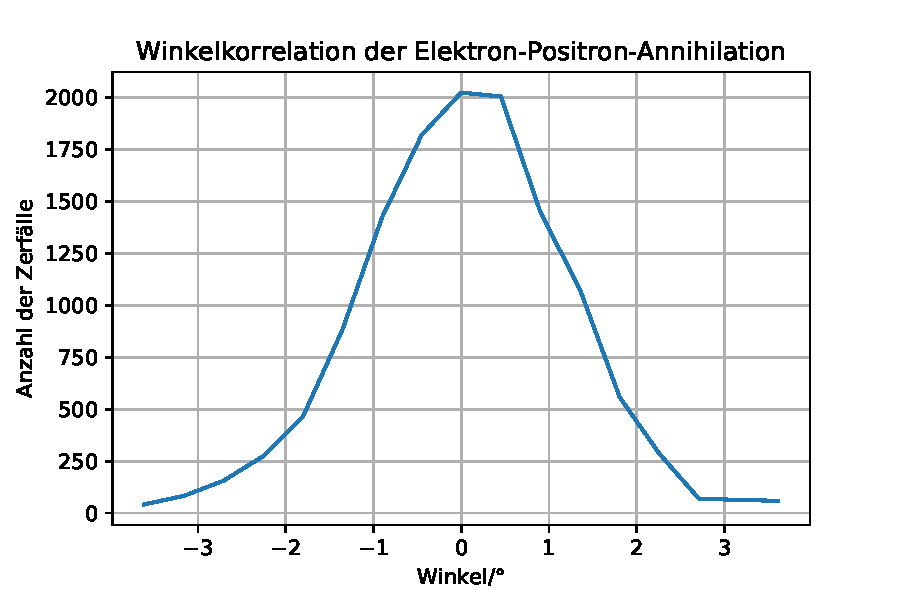
\includegraphics[width=0.7\textwidth]{Winkelkorrelation_der_Elektron-Positron-Annihilation.pdf}
  \caption{Winkelverteilung 511keV - Gammaquanten}
  \label{511}
\end{figure}

In Abbildung \ref{511} finden sich die gemessenen Zählraten abhängig des Drehwinkels des beweglichen Zählers. Wie zu erwarten findet sich um 0$^\circ$ ein scharfes Maximum, welches schon bei leichter Verschiebung des Detektors rasch abfällt. Damit ist unsere Erwartung sehr gut erfüllt und wir haben die Winkelabhängigkeit der beiden $\gamma$-Quanten sehr gut bestätigt. 

In einer weiteren Messung wird das Energiefenster des beweglichen Detektors auf den 1275keV Peak eingestellt, um auch hier die erwartete Winkelkorrelation zwischen den beiden Photonen zu erhalten. Wir erwarten allerdings keine Winkelkorrelation zwischen den Photonen, da diese ja unabhängig voneinander (eins durch die Paarvernichtung und eins durch die Abregung des Ne-Kerns) emittiert werden. Wir vermessen drei verschiedene Drehwinkel des beweglichen Detektors jeweils für 12 Minuten, um eine ausreichende Statistik zu erhalten. In Tabelle \ref{Vergleich} finden sich die gemessenen Ereignisse und wie zu erwarten sind diese für alle Winkel in etwa gleich und wir können keine Winkelkorrelation zwischen den Photonen feststellen.

\begin{table}[h]
	\caption{Winkelkorrelation unabhängiger Photonen}
	\begin{tabular}{|c|c|}
	\hline
	 Winkel & Ereignisse\\ \hline
	 30$^\circ$ & 3618 $\pm$ 60\\ \hline
	 60$^\circ$ & 3757 $\pm$ 61\\ \hline
	 90$^\circ$ & 3730 $\pm$ 61\\ \hline
	\end{tabular}
\label{Vergleich}
\end{table}

\section{Versuchsteil 2: Winkelkorrelation des $\beta$-Zerfalls von $^{60}$Co}

\subsection{Durchführung}

Wie schon im Versuchsteil 1 wird nun die Winkelverteilung zwischen den $\gamma$-Quanten des $^{60}$Co-Zerfalls gemessen. Dafür bleibt der prinzipielle Aufbau des Experiments wie in Versuchsteil 1 unverändert. Wiederum wird der Winkelbereich zwischen 0$^\circ$ und 90$^\circ$ mit 6 Messpunkten ausgemessen und die Koinzidenzzählrate sowie die Einzelzählraten bestimmt. Anschließend werden die gemessenen Winkelverteilungen einer im Kapitel 2 beschriebenen Zerfallskaskade zugeordnet und über die Einzelzählraten die Aktivität der radioaktiven Quelle bestimmt. 

\subsection{Auswertung}
Die gemessenen Zählraten abhängig des Drehwinkels des beweglichen Detektors finden sich in Tabelle \ref{Quelle}. Die Messzeit betrug dabei bei jeder Messung 700 Sekunden. Die Winkelverteilungsgröße W($\vartheta$) lässt sich dabei aus der Koinzidenzzählrate über die erwartete Winkelverteilung der zugrunde liegenden Kaskade berechnen. So entspricht W($\vartheta$) bei einem Winkel von 55$^\circ$ und einer angenommen 4-2-0-Kaskade exakt 1. Somit lassen sich die anderen gemessenen Zählungen auf diesen Wert normieren und W($\vartheta$) berechnen. Der Zusammenhang mit der Quellstärke Q ist dann folgendermaßen gegeben:

\begin{align}
\frac{Z_{12}}{Z_1Z_2}=\frac{1}{2Q}W(\vartheta)
\end{align}

\begin{table}[h]
	\caption{Messungen zur Winkelkorrelation von $^{60}$Co}
	\begin{tabular}{|c|c|c|c|c|c|}
	\hline
	 Winkel & Koinzidenzereignisse & Zähler 1 & Zähler 2 & W($\vartheta$) & Q\\ \hline
	 10$^\circ$ & 1150 & 275023 & 290139 & 1,028 & 50935\\ \hline
	 30$^\circ$ & 1190 & 277652 & 291403 & 1,063 & 51646\\ \hline
	 45$^\circ$ & 1124 & 286403 & 298235 & 1,004 & 54522\\ \hline
	 55$^\circ$ & 1119 & 280455 & 293102 & 1 & 52471\\ \hline
	 75$^\circ$ & 1039 & 281196 & 296322 & 0,929 & 53188\\ \hline
	 90$^\circ$ & 1102 & 284686 & 293432 & 0,985 & 53323\\ \hline
	\end{tabular}
\label{Quelle}
\end{table}

Die Winkelkorrelation der gemessenen Koinzidenzereignisse ist zusammen mit der Winkelverteilung für die 4-2-0-Kaskade in \ref{Co60} dargestellt. Wie zu erkennen, passen die beiden Verteilungen recht gut zueinander, sodass unsere Annahme, die Winkelverteilung einer 4-2-0-Kaskade vorliegen zu haben, bestätigt wurde. 


\begin{figure}[htbp]  
     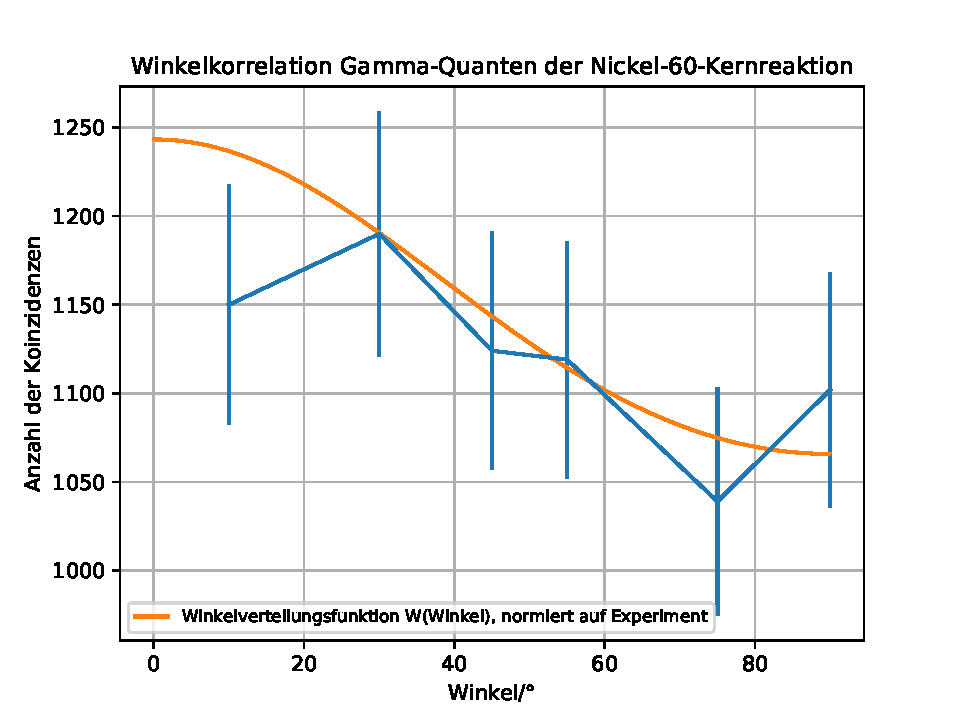
\includegraphics[width=0.7\textwidth]{Winkelkorrelation_Gamma-Quanten_der_Nickel-60-Kernreaktion.pdf}
  \caption{Winkelkorrelation $^{60}$Co-Quanten mit 4-2-0-Kaskade}
  \label{Co60}
\end{figure}

\paragraph{Bestimmung der Aktivität}



\section{Zusammenfassung/Fazit}



\bibliography{Literaturverzeichnis}
\end{document}